\documentclass{article}

\usepackage[utf8]{inputenc}
\usepackage[margin=1in]{geometry}
\usepackage{amsmath}
\usepackage{relsize}
\usepackage{hyperref}
\usepackage{dsfont}
\usepackage{graphicx}

\title{ORIE 4741: Final Report (Fairbnb)}
\author{Eric Lin (esl89), Alan Wu (ajw238), Ju Hee Lee (jl2755)}
\date{\today}
\setlength{\parindent}{0pt}

\begin{document}
\maketitle

\section{Introduction}

In recent years, we’ve seen a dramatic increase in Airbnb listings as an alternative to hotels for travelers, due to their convenience and wider outreach. Hosts can turn the homes they own into an overnight stay for traveling guests, by setting a predetermined fee and rules.
\\ \\
As the market for Airbnb listings grows, it is important to create a standardized model to predict a reason- able price for each listing, where reasonable is defined as a good compromise between the host and guest. In short, the question is "How do we determine a good price for an Airbnb listing?" This will help both parties alike, as hosts will not feel that they are charging less than they should for their listing to maximize profit, and guests will feel that they are paying an appropriate price, promoting an overall happier transaction.
\\ \\
Here we introduce Fairbnb, a play on the words Fair and Airbnb. We defined fair above to vaguely mean something like "a price that both the host and guest would be willing to pay". In fact, our dataset does not have a direct way to extract the price of a listing at the time of booking, so there is no way to tell whether a listing was booked at the price point listed. Thus, we define "fair" to mean "Given a listing with various attributes and properties, what would the average market price be?" Our goal for this project is to train a model to predict these fair prices, perhaps for a new guest who is unsure if they are getting their money's worth, or for a new host who wants to know how much their listing is worth.

\subsection{Airbnb}
Airbnb is an online marketplace for people to list and book listings around the world. Hosts can sign up with Airbnb and offer space in their properties and homes for guests to stay in. Since its start in 2008, Airbnb has hosted over 60 million guests in over 191 countries, with over 2 million listings worldwide. 


\section{Dealing With Data}
\subsection{Data Source}
The dataset that we used is provided by Inside Airbnb (\url{http://insideairbnb.com/get-the-data.html}), which is a non-commercial set of data on Airbnb listings. Here, the data contains various metrics on listings in the area such as price per night, minimum nights, intended guests, bed and bathrooms, etc. In addition, beyond having information about the housing, there are also records of number of bookings, reviews, and other relevant information from guests.

\subsection{Data Selection}
Of the many cities listed on Airbnb’s dataset, our team picked Los Angeles to fit a model on. LA is a popular destination for tourists, which means that there is plenty of data for training and testing (to be specific, about 26,000 listings). 

\subsection{Data Cleaning}
The original data set is big and messy. A lot of columns have gaps in them, and the data is not presented in a form that can be easily consumed by statistical models. We attempted to clean the data under the following principles of turning everything into an integer, and removing unnecessary columns. As a group, we decided on these criteria when it came to removing columns, since the original data had a lot to begin with (94 features):

\begin{itemize}
	\item Could this data be converted into a number easily? This meant removing text items (comments on reviews) and anything that was related to pictures, since we did not have any tools for analyzing such data.
    \item Is the data relevant to analysis at all? This prompted the removal for a lot of metadata (host name, home name, IDs, etc.) In addition, we removed everything that had to do with location since we had agreed on LA as our location already.
    \item Is the data feasible to process given its current state? Would we be able to include this within the feasibility scope of our project? Some data features had too many gaps to be valid as a feature, so we went ahead and removed those as well.
\end{itemize}

While we understand that there are lots of sentiment analysis packages out there that could have probably been used to try and classify reviews into positives or negatives, a majority of the data did not include review comments, and it felt improper to arbitrarily assign a value to such listings. In addition, the data also contains quantitative review scores for tenants that have left feedback, which we felt was sufficient for the purposes of this project.
\\ \\
A finalized list of columns that we originally decided on can be found in our \texttt{scripts} directory, under \texttt{columns\_to\_keep.txt}, with about half the original features cut. From then on, we moved on to preprocess the data.

\subsection{Data Preprocessing}
Columns (features) that are numerically-valued we will leave as is. Features that are boolean (t or f) will be converted into 0 for false and 1 for true. There are several other kinds of features that will be engineered manually, for example \texttt{host\_verifications} which is a list of the methods in which the host verified him or herself. We will either convert the list to a number representing the size, or a sum of weights where each type of verification is associated a weight.
\\ \\
In addition, there were a few feature columns that were nominal values, which we encoded using the one-hot encoding technique learned in class. Currently, we have 74 total features, with about 26000 data points. Although the number of features is quite high, there are enough data points to compensate for it, and there are no gaps in the data as well (empty features).

\subsection{Tools Used}
For preprocessing, we used Python's pandas library to handle the data (see \texttt{cleanup.py}). Pandas is something that requires additional installation past the default python packages, for those interested in replicating our data cleanup process.

\section{Evaluation Method}
\subsection{Programming Techniques}
As a brief summary, we used the Dataframes and proxgrad libraries primarily in our code. Initially we split our data into training data and a 20\% testing holdout, and we do not touch the holdout until the very end. We then construct several sets of columns that we wish to test, and run them through several different regressions via k-fold validation (we perform the regression using the proxgrad function provided). Finally we calculate the testing error for each set of columns and plot the results.

\subsection{Column Selection}
Initially, we decided to arbitrarily run a simple linear regression using all 79 features. This resulted in a large significant error when running it on the testing set, as well as very large weights on some interesting columns that we did not expect to be relevant. For example, one of the largest weights was longitude, for example, which we did not expect to have any effect on the pricing, being that every listing in Los Angeles should have more or less the same longitude.

To accommmodate for this, and to prevent ourselves from using all 79 features of data, we experimentally decided to use groups of features that we believed would have some inherent effect on pricing. After 6 rounds of random sampling and testing (columns are described in greater detail below), we decided on a meaningful group of columns. The column groupings are as follows, with \texttt{columns\_6} being our final version of what we experimented on.

\begin{verbatim}
columns_1 = [:accommodates, :beds, :amenities, :review_scores_rating, :offset]
columns_2 = [:accommodates, :beds, :offset]
columns_3 = [:accommodates, :beds, :room_type_entire_home_apt, :offset]
columns_4 = [:accommodates, :beds, :room_type_entire_home_apt, :reviews_per_month, :offset]
columns_5 = [:accommodates, :beds, :bed_type_real_bed, :room_type_entire_home_apt, 
    		:reviews_per_month, :property_type_apartment, :offset]
columns_6 = [:accommodates, :beds, :bed_type_real_bed, :room_type_entire_home_apt, 
    		:room_type_private_room, :room_type_shared_room, 
    		:reviews_per_month, :property_type_apartment, :offset]
\end{verbatim}
 
\subsection{Overfitting and Underfitting}
After coming up with a few different models for our data, we may run into cases of overfitting or underfitting. Overfitting is when the model performs well on the training data, but does not generalize well to other data. Underfitting is when the model performs poorly on the training data, and also does not generalize well to other data. Both scenarios should not happen with well-fitted models. To detect overfitting, we can use cross validation to calculate the average validation error. There are several methods to reduce overfitting. The two methods that we are going to consider are \textit{k-fold validation} and \textit{regularization}. Underfitting means that there is high bias. For our project, we are unlikely to run into underfitting because our data set is quite large. In the case of underfitting, we could experiment with which features we are going to include for our model. The selection of features is important to come up with an optimal model.

\section{Experimentation Method}
For our Fairbnb Model, we used multiple linear regression, which predicts the value of one dependent variables using two or more independent variables. Let $X \in \mathds{R}^{n \times d}$ be the training data which contains n listings with d features. Let $Y \in \mathds{R}^{d}$ be the price for each listing in the training data. Let $w \in \mathds{R}^{d}$ be the linear model coefficients computed using some regression model. We experimented by filtering our data set with different sets of independent variables/columns, as well as different types of loss functions and regularizers. The regularizers we used were No regularizer, L1, and L2 which are all commonly used. These experiments are explained in more detail in the following sections.

\begin{equation}
	h(x) = w_1*x_1 + w_2*x_2 + ... + w_d*x_d
\end{equation}

In order to determine the accuracy of each model, we used the Root Means Squared Error on our test set as follows:

\begin{align*}
  RMSE(X,y,w) = \sqrt{\mathlarger{\mathlarger{\sum}}_{x \in X} (y-w^T x)^2}
\end{align*}

\subsection{Different Loss Functions}

We decided to experiment with some commonly used regression loss functions: Huber, Quadratic, and L1 Loss. For each of these regressions, we explored the option of adding regularizers. For all three graphs, the y-axis is the root-mean-squared-error. For each type of loss and regularizer, we plotted the testing error of each of the 6 datasets filtered by selected columns. 


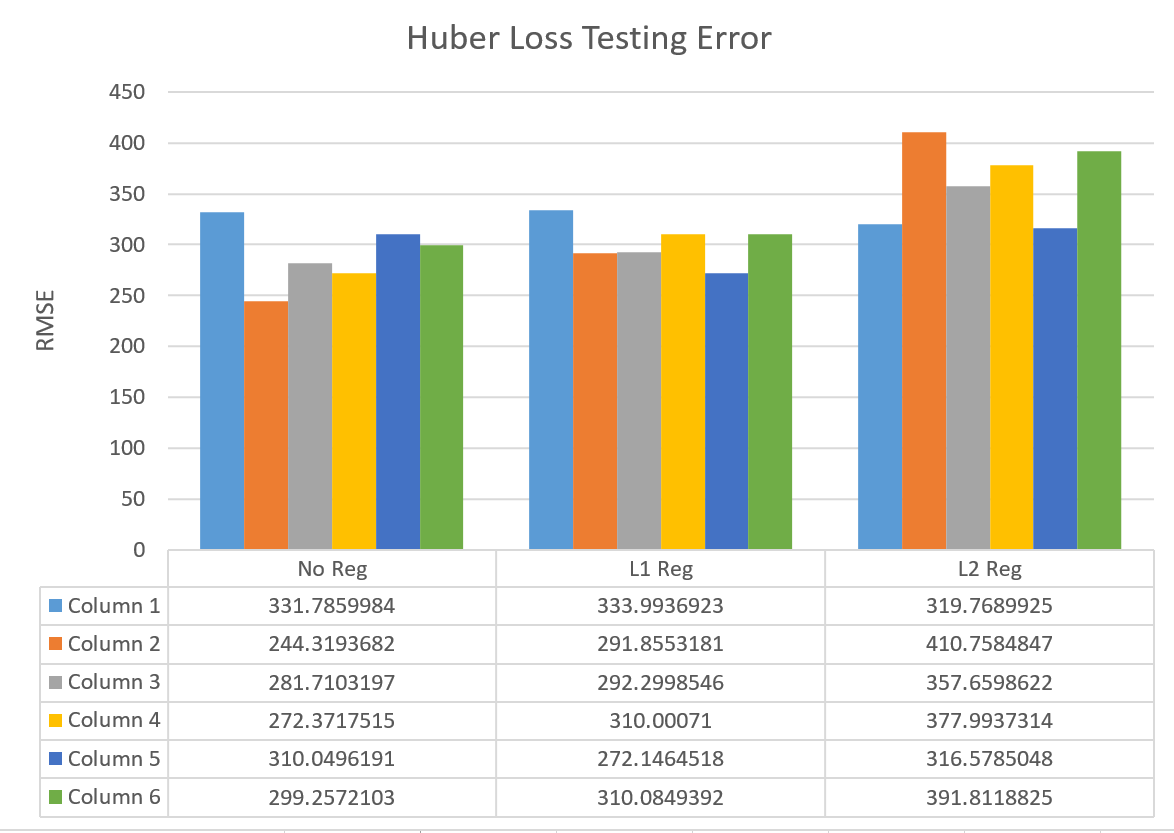
\includegraphics[width=\textwidth]{HuberLoss}
Huber Loss, also known as Smooth Absolute Loss, is defined as the following.

  \begin{equation}
    l(x_i, y_i; h_w)=
    \begin{cases}
      \frac{1}{2}(h_w(x_i) - y_i)^2, & \text{if}\  \mid h_w(x_i) - y_i \mid < \delta \\
      \delta(\mid h_w(x_i) - y_i \mid - \delta/2), & \text{otherwise}
    \end{cases}
  \end{equation}
  
Huber Loss has the advantage of squared and absolute loss. When the difference between the expected and actual value is small, the loss is squared. Otherwise, the absolute difference is added to the loss. Huber loss is once differentiable, and takes on the behavior of squared-loss when the loss is small, and absolute loss when the loss is large. 

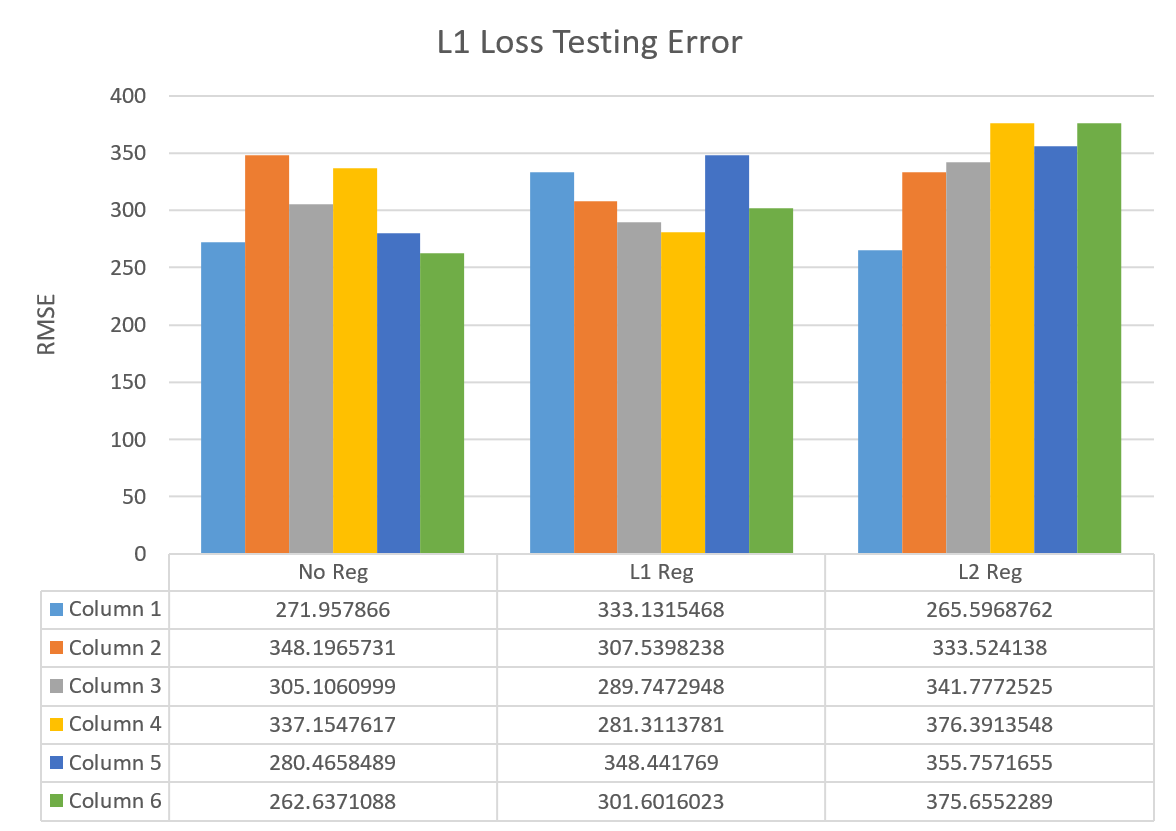
\includegraphics[width=\textwidth]{L1Loss}
	\begin{equation}
    	l(x_i, y_i; h_w) = |h_w(x_i) - y_i|
    \end{equation}
    
L1 Loss, also known absolute loss, minimizes the sum of absolute differences between the expected and the actual values. It is a popular loss function, and it estimates the median label. An advantage is that it is less sensitive to noise, but it is not differentiable at 0.
    
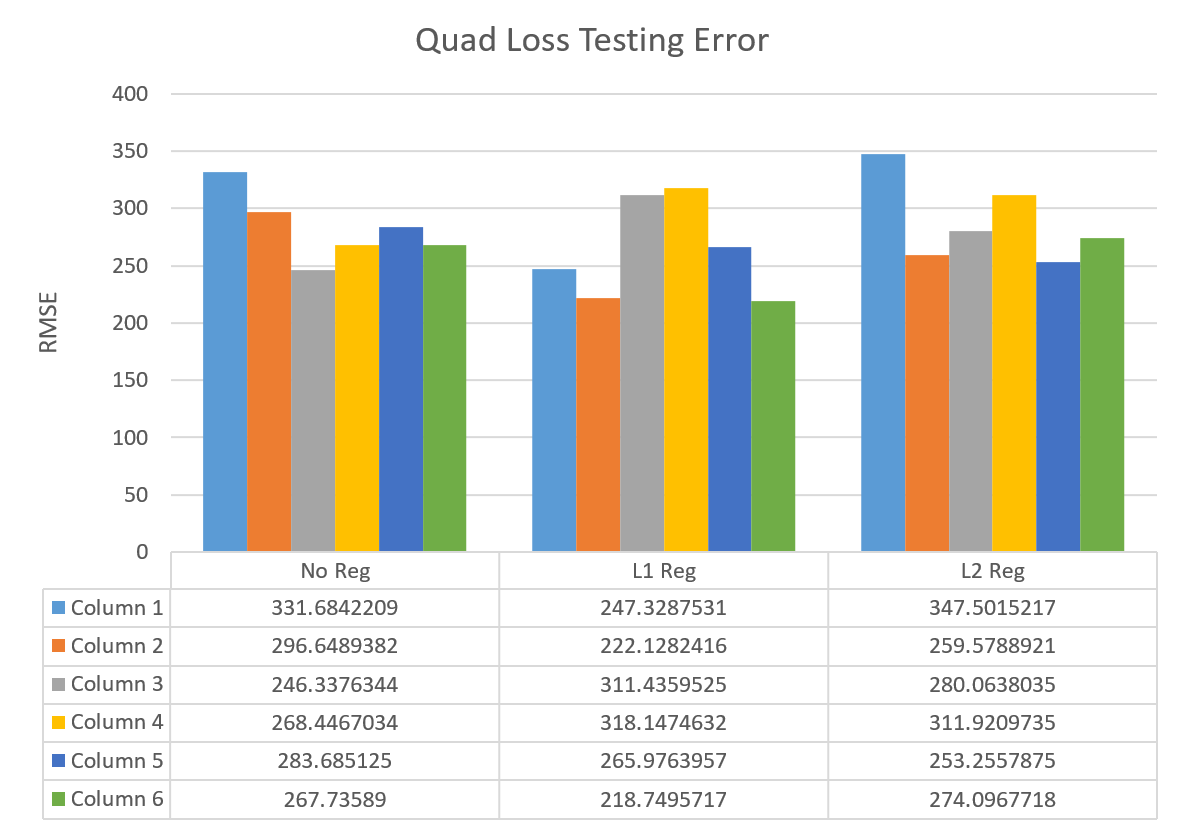
\includegraphics[width=\textwidth]{QuadLoss}
	\begin{equation}
    	l(x_i, y_i; h_w) = (h_w(x_i) - y_i)^2
    \end{equation}
    
Quad Loss, also known as Ordinary Least Squares (OLS), is used to minimize the sum of squared differences between the expected and the actual values. It is the most popular regression loss function, and it estimates the mean label. This loss function is differentiable everywhere, but it is sensitive to outliers and noise.


\subsection{K-Fold Cross Validation and Bootstrapping}
In an effort to reduce overfitting on our training set, we implemented k-fold validation as follows. Each of the k iterations, we split the data (ignoring the test set) into training and validation sets based on an upper and lower bound of indices (and put the rest into validation), train a model, and then add the weights to an average. At the end we divide the weights by the number of folds.
\\ \\
We also implemented random bootstrapping on our models to reduce variance. It performs the same procedure as above, but randomly splits the data into a training and validation set k times, then averages the results. 


\section{Results and Analysis}
\subsection{Significant Features}
Once we trained a model on our data, we proceeded to test it on the 20\% testing holdout data. We used root-mean-squared-error to calculate our error rate. When we examined our models more closely, we noticed that the most prominent features were 
\begin{enumerate}
\item number of people to accommodate
\item number of beds. 
\item bed type (real bed, couch, futon, etc.)
\item room type (entire home)
\end{enumerate}

After running Huber loss on our data set that was filtered by the columns (defined in columns\_6 below), we saw that these four features the most positive coefficients. The rest of the coefficients, besides the intercept, were negative and had smaller absolute values. This aligned with our predictions because houses that hold more people tend to be more expensive, and customers prefer having real beds and an entire home, rather than a shared or private room.
\begin{verbatim}
columns_6 = [:accommodates, :beds, :bed_type_real_bed, :room_type_entire_home_apt, 
    		:room_type_private_room, :room_type_shared_room, 
    		:reviews_per_month, :property_type_apartment, :offset]
w_huber6 = [27.6407,10.32,9.56071,19.5859,-4.42984,-5.61282,-3.46036,-1.8494,9.54327]
\end{verbatim}

\subsection{Final Model}
After all the experiments, the model that used Quad loss with L1 regularizer had the lowest root-mean-squared-error of \textbf{218.74}. When we observed the weights of $w$, we saw similarities and differences from the weight vector computed using Huber loss. Just like the Huber model, the number of people to accommodate, the number of beds, and the room type being an entire home or apartment contributed positively to the price of the house. On the other hand, whether the bed was a "real bed" contributed neither positively nor negatively to the price of the house. The coefficients for rest of the features in columns\_6 were all negative just like the Huber model, but they had larger absolute values. The coefficients of the features ``room type private room'' and ``room type shared room'' were negative, which aligned with our prediction because customers prefer entire homes or apartments. The coefficients for ``reviews per month'' and ``property type apartment'' were also very negative. Initially, we thought that having higher reviews per month would lead to a higher price. However, we realized that having higher reviews does not necessarily mean that the house is more expensive. Airbnb customers often look for cheaper options than staying at expensive hotels. Thus, a cheap Airbnb listing could easily receive high ratings if it offered cleanliness, safety, and convenient location to the customer's satisfaction.

\begin{verbatim}
w1_quad6 = [55.3715,19.3343,0.0,22.4788,-6.17719,-17.2705,-20.1734,-44.4788,-1.4063]
\end{verbatim}

\subsection{Takeaways}
In our attempt to try and model Airbnb prices, we created various models that generally ended up with the same amount of error when running it against our testing set. While it was unfortunate that we were unable to create a valid model for production, we are quite confident with our analysis from a technical standpoint; nothing that we had done had any errors in it, but perhaps the nature of the data and models themselves accounted for such a disparity. Therefore, we would not recommend this model be placed in production, due to the model not being completely accurate. This is under the assumption that the current Airbnb listings market is already fairly priced (for the listings that are rented).

\end{document}
